\documentclass[]{beamer}

% File: preamble.tex
\usepackage{lmodern}

% \usepackage{xeCJK}
\usetheme{CambridgeUS} % try Pittsburgh
\usecolortheme{beaver}
\usefonttheme[onlymath]{serif} % try "professionalfonts"

\setbeamertemplate{itemize items}[default]
\setbeamertemplate{enumerate items}[default]

\usepackage{amsmath, amsfonts, latexsym, mathtools, tabu}
\newcommand{\set}[1]{\left\{#1\right\}}
\newcommand{\ps}[1]{\mathcal{P}(#1)}
\usepackage{bm}
\DeclareMathOperator*{\argmin}{\arg\!\min}
\DeclareMathOperator*{\E}{\mathbb{E}}

\usepackage{algorithm}
\usepackage[noend]{algpseudocode}
\newcommand{\hStatex}[0]{\vspace{5pt}}

% colors
\newcommand{\red}[1]{\textcolor{red}{#1}}
\newcommand{\redoverlay}[2]{\textcolor<#2>{red}{#1}}
\newcommand{\green}[1]{\textcolor{green}{#1}}
\newcommand{\greenoverlay}[2]{\textcolor<#2>{green}{#1}}
\newcommand{\blue}[1]{\textcolor{blue}{#1}}
\newcommand{\blueoverlay}[2]{\textcolor<#2>{blue}{#1}}
\newcommand{\purple}[1]{\textcolor{purple}{#1}}
\newcommand{\cyan}[1]{\textcolor{cyan}{#1}}
\newcommand{\violet}[1]{\textcolor{violet}{#1}}
\newcommand{\lgray}[1]{\textcolor{lightgray}{#1}}
\newcommand{\teal}[1]{\textcolor{teal}{#1}}
\newcommand{\brown}[1]{\textcolor{brown}{#1}}

\newcommand{\wlspec}{$\mathcal{A}_{\text{weak}}$}

% colorded box
\newcommand{\rbox}[1]{\red{\boxed{#1}}}
\newcommand{\gbox}[1]{\green{\boxed{#1}}}
\newcommand{\bbox}[1]{\blue{\boxed{#1}}}
\newcommand{\pbox}[1]{\purple{\boxed{#1}}}

\usepackage{pifont}
\usepackage{wasysym}

\newcommand{\cmark}{\green{\ding{51}}}
\newcommand{\xmark}{\red{\ding{55}}}
%%%%%%%%%%%%%%%%%%%%%%%%%%%%%%%%%%%%%%%%%%%%%%%%%%%%%%%%%%%%%%
\usepackage{subfig}

% for fig without caption: #1: width/size; #2: fig file
\newcommand{\fignocaption}[2]{
  \begin{figure}[htp]
    \centering
      \includegraphics[#1]{#2}
  \end{figure}
}

\usepackage{tikz}
\usetikzlibrary{positioning, mindmap, shadows, calc, arrows.meta, backgrounds, fit, shapes}


\newcommand{\push}{\texttt{Push}}
\newcommand{\pop}{\texttt{Pop}}

\newcommand{\titletext}{Specification and Implementation of Replicated List}

\newcommand{\thankyou}{
  \begin{frame}[noframenumbering]{}
    \fignocaption{width = 0.50\textwidth}{figs/thankyou.png}
  \end{frame}
}

%%%%%%%%%%
\title[Replicated List (Jupiter)]{\titletext}
\subtitle{--- The Jupiter Protocol Revisited \\[10pt] \teal{(Brief Announcement at PODC'2018)}}

\author[Hengfeng Wei]{\large {\bf Hengfeng Wei}, Yu Huang, Jian Lu}
\titlegraphic{
\includegraphics[height = 2.0cm]{figs/nju-logo-purple}}
\institute{Nanjing University}
\date{July 24, 2018}

\AtBeginSection[]{
  \begin{frame}[noframenumbering, plain]
    \frametitle{\titletext}
    \tableofcontents[currentsection, sectionstyle=show/shaded, subsectionstyle=show/show/hide]
  \end{frame}
}
%%%%%%%%%%
\begin{document}

\maketitle

% file: parts/ba.tex

%%%%%%%%%%%%%%%%%%%%
\begin{frame}{}
  \begin{center}
    {\large We claim one thing in this BA:} \\[10pt]

    {\Large The \blue{Jupiter} protocol~\ncite{Nichols:UIST95}\footfullcite{Nichols:UIST95} for replicated list \\
    \red{satisfies} the \blue{weak list specification}~\ncite{Attiya:PODC16}\footfullcite{Attiya:PODC16}.}  \\[25pt]

    \pause
    {\large This was proposed as a conjecture in a PODC paper~\ncite{Attiya:PODC16}.}
  \end{center}
\end{frame}
%%%%%%%%%%%%%%%%%%%%


% file: parts/overview.tex

%%%%%%%%%%%%%%%%%%%%
\begin{frame}{}
  \centerline{\Huge \teal{Background}}
\end{frame}
%%%%%%%%%%%%%%%%%%%%

%%%%%%%%%%%%%%%%%%%%
\begin{frame}{}
  \centerline{\large \teal{\red{Replicated}, highly available collaborative text editing systems}}

  \fignocaption{width = 0.55\textwidth}{figs/coeditor}

  \pause
  \vspace{-0.50cm}
  \begin{center}
    Replicas are required to respond to user operations \red{immediately}.  \\[3pt]

    Updates are propagated to other replicas \red{asynchronously}.
  \end{center}
\end{frame}
%%%%%%%%%%%%%%%%%%%%

%%%%%%%%%%%%%%%%%%%%
\begin{frame}{}
  \centerline{\Large \red{Replicated list object}: to model the core functionality}
  \vspace{0.30cm}

  \begin{center}
    \begin{minipage}{0.70\textwidth}
      \begin{description}
	\setlength{\itemsep}{10pt}
	\item[$\textsc{Ins}(a, p):$] Insert $a$ at position $p$.
	\item[$\textsc{Del}(p):$] Delete the element at position $p$.
	\item[$\textsc{Read}:$] Return the list.
      \end{description}
    \end{minipage}
  \end{center}
\end{frame}
%%%%%%%%%%%%%%%%%%%%

%%%%%%%%%%%%%%%%%%%%
\begin{frame}{}
  \begin{definition}[Eventual Convergence (EC)~\ncite{Ellis:SIGMOD89}]
    The lists at all replicas are identical \purple{\it at quiescence}.
  \end{definition}

  \vspace{0.50cm}

  % \vspace{-0.50cm}
  % \fignocaption{width = 0.25\textwidth}{figs/specs}
  % \vspace{-0.50cm}

  \begin{definition}[Strong Eventual Consistency (SEC)~\ncite{Shapiro:SSS11}]
    The lists at the replicas that \purple{\it have executed the same set of user operations} are identical.
  \end{definition}

  \vspace{1.00cm}
  \centerline{\red{\large Specify little on \teal{\it intermediate states} going through by replicas.}}
\end{frame}
%%%%%%%%%%%%%%%%%%%%

%%%%%%%%%%%%%%%%%%%%
\begin{frame}{}
  \begin{center}
    \red{\large Strong/weak list specification}~\ncite{Attiya:PODC16} \\[6pt]
    \teal{Specify global properties on all states at all replicas.}
  \end{center}

  \fignocaption{width = 0.80\textwidth, frame}{figs/podc16-attiya}

  \pause
  \vspace{0.50cm}
  \begin{center}
    \begin{description}
      \item[Proved:] RGA~\ncite{Roh:JPDC11} satisfies the strong list specification.
      \item[Conjecture:] \red{Jupiter}~\ncite{Nichols:UIST95} satisfies the weak list specification.
    \end{description}
  \end{center}
\end{frame}
%%%%%%%%%%%%%%%%%%%%

% file: parts/problem.tex

%%%%%%%%%%%%%%%%%%%%
\begin{frame}{}
  \centerline{\Huge \teal{Problem}}
\end{frame}
%%%%%%%%%%%%%%%%%%%%

% file: parts/wlspec.tex

%%%%%%%%%%%%%%%%%%%%
\begin{frame}{}
  \centerline{\Huge \teal{Weak List Specification}}
\end{frame}
%%%%%%%%%%%%%%%%%%%%

%%%%%%%%%%%%%%%%%%%%
\begin{frame}{}
  \begin{definition}[Weak List Specification \wlspec{}~\cite{Attiya:PODC16}]
    Informally, \wlspec{} requires the ordering between \red{elements that are not deleted} to be consistent across the system.
  \end{definition}

  \pause
  \vspace{1.00cm}
  \begin{definition}[Pairwise State Compatibility Property]
    \[
      \forall \sigma, \sigma': a, b \in \sigma \cap \sigma' \implies (a \prec_{\sigma} b \iff a \prec_{\sigma'} b)
    \]
  \end{definition}
\end{frame}
%%%%%%%%%%%%%%%%%%%%

%%%%%%%%%%%%%%%%%%%%
\begin{frame}{}
  \begin{definition}[Pairwise State Compatibility Property]
    \[
      \forall \sigma, \sigma': a, b \in \sigma \cap \sigma' \implies (a \prec_{\sigma} b \iff a \prec_{\sigma'} b)
    \]
  \end{definition}

  \vspace{0.60cm}
  \begin{columns}
    \column{0.50\textwidth}
      \pause
      \fignocaption{width = 0.60\textwidth}{figs/ex-weak-list-spec}
      \vspace{-0.60cm}
      \fignocaption{width = 0.40\textwidth}{figs/red-cross}
    \column{0.50\textwidth}
      \pause
      \fignocaption{width = 0.75\textwidth}{figs/ex-strong-list-spec}
      \vspace{-0.60cm}
      \fignocaption{width = 0.30\textwidth}{figs/green-check}
  \end{columns}
\end{frame}
%%%%%%%%%%%%%%%%%%%%

% file: parts/jupiter.tex

%%%%%%%%%%%%%%%%%%%%
\begin{frame}{}
  \centerline{\Huge \teal{Jupiter}}
\end{frame}
%%%%%%%%%%%%%%%%%%%%

%%%%%%%%%%%%%%%%%%%%
\begin{frame}{}
  \begin{columns}
    \column{0.50\textwidth}
      \begin{center}
	% file: tikz/jupiter-cs-tikz.tex

\def\s{s}  % server
\def\b{bot} % literal string
\tikzset{seq/.style = {draw, circle, outer sep = 5pt, inner sep = 2pt, scale = #1, left}}

% send: the sender sends operation to the receiver
\newcommand{\send}[5]{% #1: sender; #2: receiver; #3: sender pos; #4: receiver pos; #5: seq. number;
  \draw[->]  ($(#1)!#3!(#1\b)$) node[seq = 0.40] {#5} to ($(#2)!#4!(#2\b)$) node[seq = 0.60] {$#5$};
}

% csend: client sends operation to the server
\newcommand{\csend}[6]{% #1: client; #2: client pos; #3: server pos; #4: seq. number; #5: client state; #6: server state
  \draw[->]  ($(#1)!#2!(#1\b)$) node[seq = 0.60, draw = none] (#4) {} to ($(\s)!#3!(\s\b)$) {};
}

% ssend: the server sends operation to client 
\newcommand{\ssend}[5]{% #1: client; #2: server pos; #3: client pos; #4: seq. number; #5: client state
  \draw[->, dashed]  ($(\s)!#2!(\s\b)$) to ($(#1)!#3!(#1\b)$) node[solid, seq = 0.60] {$#4$};
}

\newcommand{\ins}[2]{$\textcolor{blue}{\textsc{Ins}(#1,#2)}$}
\newcommand{\del}[2]{$\textcolor{blue}{\textsc{Del}(#2)}$}  % del(a,p): ignoring the element 'a'

\begin{tikzpicture}[
    timeline/.style = {very thick}, >=Stealth, 
    op/.style = {font = \small, above left = -0.20cm and -0.40cm of #1, sloped},
    replica/.style = {align = center}]
  \uncover<1->{
    \node[replica] (\s) {\textcolor{brown}{$S$}};
    \node[replica, right = of s] (c1) {$\textcolor{brown}{C_1}$};
    \node[replica, right = of c1] (c2) {$\textcolor{brown}{C_2}$};
    \node[replica, right = of c2] (c3) {$\textcolor{brown}{C_3}$};

    \foreach \r/\rbot in {s/sbot, c1/c1bot, c2/c2bot, c3/c3bot} {
	  \node[below = 5.0cm of \r] (\rbot) {};
	  \draw[timeline] (\r) to (\rbot);
    }
  }

  \uncover<2->{
    % Clients send messages (ordered by positions at server) to the server
    \csend{c1}{0.15}{0.20}{1}{x}{x}
    \csend{c1}{0.35}{0.40}{2}{}{}
    \csend{c2}{0.45}{0.55}{3}{ax}{a}
    \csend{c3}{0.50}{0.75}{4}{xb}{}
  }

  \uncover<3->{
    % Operations are totally ordered at the server.
    \foreach \num/\pos in {1/0.20, 2/0.40, 3/0.55, 4/0.75} {
      \node [seq = 0.80, fill = red!40] at ($(\s)!\pos!(\s\b)$) {$\num$};
    }
  }

  % \node (o1) [op = {1}, rotate = 7] {};
  % \node (o2) [op = {2}, rotate = 7] {};
  % \node (o3) [op = {3}, rotate = 8] {};
  % \node (o4) [op = {4}, rotate = 15] {};

  \uncover<4->{
    % The server sends messages (ordered by positions at server) to clients.
    \ssend{c2}{0.40}{0.65}{2}{a}
    \ssend{c3}{0.40}{0.70}{2}{b}

    \ssend{c2}{0.20}{0.30}{1}{x}
    \ssend{c3}{0.20}{0.25}{1}{x}


    \ssend{c1}{0.55}{0.60}{3}{a}
    \ssend{c3}{0.55}{0.90}{3}{}

    \ssend{c1}{0.75}{0.90}{4}{}
    \ssend{c2}{0.75}{0.90}{4}{}
  }
\end{tikzpicture}

      \end{center}
    \column{0.45\textwidth}
      System model of Jupiter~\ncite{Nichols:UIST95}: \\[5pt]
      \begin{itemize}
	\setlength{\itemsep}{10pt}
	\item<1-> client-server architecture
	\item<2-> client $\xrightarrow[]{\quad \text{FIFO} \quad}$ server
	\item<3-> totally ordered at the server
	\item<4-> server $\xrightarrow[]{\quad \text{FIFO} \quad}$ client
      \end{itemize}
  \end{columns}
\end{frame}
%%%%%%%%%%%%%%%%%%%%

%%%%%%%%%%%%%%%%%%%%
\begin{frame}{}
  \centerline{OT (Operational Transformation)~\ncite{Ellis:SIGMOD89}}

  \begin{columns}[c]
    \column{0.50\textwidth}
      \fignocaption{width = 0.70\textwidth}{figs/ot-tcs06}
    \column{0.50\textwidth}
      \pause
      \fignocaption{width = 0.65\textwidth}{figs/ot}
      \[
	\sigma; o_1; o_2' \equiv \sigma; o_2; o_1'
      \]
  \end{columns}
\end{frame}
%%%%%%%%%%%%%%%%%%%%

%%%%%%%%%%%%%%%%%%%%
\begin{frame}{}
  \begin{center}
    {\large Jupiter uses \red{$2D$ state spaces}~\ncite{Sun:CSCW14} \\
    to manage how and when to perform OTs.}
  \end{center}

  \fignocaption{width = 0.35\textwidth}{figs/2d-statespace}

  \begin{center} 
    \pause
    Nodes represent states. \quad Edges are labeled with operations.

    \pause
    \red{$2D$}: An operation from the same node is either \textsc{Local} or \textsc{Global}. 
  \end{center}
\end{frame}
%%%%%%%%%%%%%%%%%%%%

%%%%%%%%%%%%%%%%%%%%
\begin{frame}{}
  \centerline{\large Each \red{client} maintains a $2D$ state space.}

  \fignocaption{width = 0.50\textwidth}{figs/jupiter-illustration-client3-notations}

  \centerline{\large The \red{server} maintains $n \; (=3)$ $2D$ state spaces, one for each client.}
\end{frame}
%%%%%%%%%%%%%%%%%%%%

%%%%%%%%%%%%%%%%%%%%
\begin{frame}{}
  \begin{center}
    {\large \red{Global property} on all replica states \\ specified by the \blue{weak list specification}}

    \vspace{0.20cm}
    \fignocaption{width = 0.30\textwidth}{figs/mismatch}
    \vspace{0.20cm}

    {\large \red{Local view} each replica maintains in \blue{Jupiter}}
  \end{center}
\end{frame}
%%%%%%%%%%%%%%%%%%%%

% file: parts/cjupter.tex

%%%%%%%%%%%%%%%%%%%%
\begin{frame}{}
  \centerline{\Huge \teal{CJupiter (Compact Jupiter)}}
\end{frame}
%%%%%%%%%%%%%%%%%%%%

%%%%%%%%%%%%%%%%%%%%
\begin{frame}{}
  \begin{center}
    {\large CJupiter maintains an \red{$n$-ary ordered state space} for each replica.}
  \end{center}

  \fignocaption{width = 0.40\textwidth}{figs/cjupiter-allinone}

  \begin{center} 
    There can be \red{more than two edges} coming from the same node. \\[5pt]
    Edges from the same node are \red{totally ordered} by associated operations.
  \end{center}
\end{frame}
%%%%%%%%%%%%%%%%%%%%

%%%%%%%%%%%%%%%%%%%%
\begin{frame}{}
  \begin{center}
    \begin{prop}[Compactness of CJupiter (Informal)]
      {\large At a high level, CJupiter maintains only \red{one} $n$-ary ordered state space.}
    \end{prop}

    \vspace{0.20cm}
    % \resizebox{0.50\textwidth}{!}{% file: tikz/cjupiter-allinone-path.tex
% CSS lattice for jupiter-scheduling-podc16.tex

% default horizontal/vertical distance
\def\hdist{1.8}
\def\vdist{1.8}

\newcommand{\state}[2]{% #1: state label; #2: position
  \node (#1) [circle, inner sep = 0pt, minimum size = 10mm, text width = 10mm, align = center, draw, #2, font = \Large] {$#1$};
}

\tikzset{every lower node part/.style = {red}}
\newcommand{\statesplit}[3]{% #1: state upper label; #2: state lower label; #3: position
  \node (#1) [circle split, draw, minimum size = 6mm, text width = 10mm, align = center, #3, font = \Large]
  {
	$#1$
	\nodepart{lower}
	$#2$
  };
}

\newcommand{\transition}[4][]{% #2: start state; #3: end state; #4: transition label; #1: transition label position (optional)
  \draw[>=Stealth, ->] (#2) to node [rectangle, draw, above = 2pt, sloped, #1, font = \small] {#4} (#3);
}

\newcommand{\ins}[2]{$\textsc{Ins}(#1,#2)$}
\newcommand{\del}[2]{$\textsc{Del}(#1,#2)$}

\tikzset{node distance = \vdist and \hdist}
\tikzset{path/.style = {draw, rounded corners, ultra thick, #1}}

\begin{tikzpicture}
  \uncover<1->{
    \statesplit{0}{\epsilon}{}
    \statesplit{1}{x}{below = of 0}
    \transition{0}{1}{1: \ins{x}{0}}

    \statesplit{12}{\epsilon}{below left = of 1}
    \statesplit{13}{ax}{below right = of 1}
    % \statesplit{123}{a}{below = 2.1*\vdist of 1}
    \statesplit{123}{a}{below right = of 12}
    \transition{1}{12}{2: \del{x}{0}}
    \transition{1}{13}{3: \ins{a}{0}}
    \transition{12}{123}{3: \ins{a}{0}}
    \transition{13}{123}{2: \del{x}{1}}

    % \statesplit{14}{xb}{right = 1.5*\vdist of 13}
    % \transition{1}{14}{4: \ins{b}{1}}

    % \statesplit{124}{b}{right = 2.1*\hdist of 123}
    \statesplit{124}{b}{below right = of 13}
    \transition[near end]{12}{124}{4: \ins{b}{0}}
    
    % \statesplit{1234}{ba}{below = 2*\vdist of 13}
    \statesplit{1234}{ba}{below right = of 123}
    \transition{124}{1234}{3: \ins{a}{1}}
    \transition{123}{1234}{4: \ins{b}{0}}

    \statesplit{14}{xb}{above right = of 124}
    \transition{1}{14}{4: \ins{b}{1}}
    \transition{14}{124}{2: \del{x}{0}}
  }

  \uncover<2->{
    \path[path = {red}] ($(0.north) + (135:20pt)$) node[left] 
	  (sc1) {$S, C_1$} -- ++(-90:2.5*\vdist) -- ++(-135:2.5*\vdist) -- ++(-45:5.2*\vdist); % -- ++(-50:2.6*\vdist);
    \path[path = {blue}] ($(0.north) + (100:20pt)$) node[above = 0pt] 
	  (c2) {$C_2$} -- ++(-90:2.7*\vdist) -- ++(-45:2.5*\vdist) -- ++(-135:2.2*\vdist) -- ++(-45:2.4*\vdist);
    \path[path = {teal}] ($(0.north) + (60:15pt)$) node[right] 
	  (c3) {$C_3$} -- ++(-90:2.5*\vdist) -- ++(-18:5.5*\vdist) -- ++(-135:5.0*\vdist);
  }
\end{tikzpicture}}
    \fignocaption{width = 0.40\textwidth}{figs/cjupiter-allinone-path}

    \vspace{0.20cm}
    Each replica behavior corresponds to a \red{path} going through this state space.
  \end{center}
\end{frame}
%%%%%%%%%%%%%%%%%%%%

%%%%%%%%%%%%%%%%%%%%
\begin{frame}{}
  \begin{Theorem}[Equivalence of CJupiter and Jupiter]
    Under the same schedule, the behaviors of corresponding replicas in CJupiter and Jupiter are the same.
  \end{Theorem}

  \vspace{1.0cm}
  \centerline{\large From the perspectives of both the server and the clients.}
\end{frame}
%%%%%%%%%%%%%%%%%%%%

% file: parts/sat-proof.tex

%%%%%%%%%%%%%%%%%%%%
\begin{frame}{}
  \centerline{\teal{\Large \red{CJupiter} satisfies the weak list specification.}}
\end{frame}
%%%%%%%%%%%%%%%%%%%%

%%%%%%%%%%%%%%%%%%%%
\begin{frame}{}
  \begin{center}
    {\large We study \blue{a single $n$-ary ordered state space} $\text{CSS}_{s}$ at the server \\ which provides a global view of all possible replica states.}
  \end{center}

  \fignocaption{width = 0.45\textwidth}{figs/cjupiter-allinone-path}

  \pause
  \begin{center}
    {\large To show the \red{pairwise state compatibility} property \blue{in three steps}.}
  \end{center}
\end{frame}
%%%%%%%%%%%%%%%%%%%%

%%%%%%%%%%%%%%%%%%%%
\begin{frame}{}
  \centerline{\circled{1} Take any two nodes/states $v_1$ and $v_2$.}

  \begin{lemma}[LCA (Lowest Common Ancestor)]
    Each pair of states in the $n$-ary ordered state space has a \red{unique} LCA.
  \end{lemma}

  \begin{columns}
    \column{0.60\textwidth}
      \fignocaption{width = 0.50\textwidth}{figs/lca}
      \column{0.30\textwidth}
	\[
	  v_0 = \text{LCA}(v_1, v_2)
	\]
  \end{columns}

  % \fignocaption{width = 0.25\textwidth}{figs/lca}
  % \[
  %   v_0 = \text{LCA}(v_1, v_2)
  % \]
\end{frame}
%%%%%%%%%%%%%%%%%%%%

%%%%%%%%%%%%%%%%%%%%
\begin{frame}{}
  \centerline{\circled{2} Consider the paths to $v_1$ and $v_2$ from their LCA $v_0$.}

  \begin{lemma}[Disjoint Paths]
    The set of operations $O_{v_0 \leadsto v_1}$ along $P_{v_0 \leadsto v_1}$ 
    is \red{disjoint} from the set of operations $O_{v_0 \leadsto v_2}$ along $P_{v_0 \leadsto v_2}$.
  \end{lemma}

  \begin{columns}
    \column{0.60\textwidth}
	\fignocaption{width = 0.50\textwidth}{figs/disjoint-paths}
      \column{0.30\textwidth}
	\[
	  v_0 = \text{LCA}(v_1, v_2)
	\]
  \end{columns}
\end{frame}
%%%%%%%%%%%%%%%%%%%%

%%%%%%%%%%%%%%%%%%%%
\begin{frame}{}
  \centerline{\circled{3} Consider the states in these two paths.}

  \begin{lemma}[Compatible Paths]
    Each pair of states consisting of one state $v$ in $P_{v_0 \leadsto v_1}$ and the other $v'$ in $P_{v_0 \leadsto v_2}$ are \red{compatible}.
  \end{lemma}

  \begin{columns}
    \column{0.60\textwidth}
	\fignocaption{width = 0.55\textwidth}{figs/compatible-paths}
      \column{0.40\textwidth}
	\[
	  v_0 = \text{LCA}(v_1, v_2)
	\]

	\vspace{0.50cm}
	\begin{center}
	  {In particular, \\ $v_1$ and $v_2$ are compatible.}
	\end{center}
  \end{columns}
\end{frame}
%%%%%%%%%%%%%%%%%%%%


\thankyou{}
% file: parts/bib.tex

%%%%%%%%%%%%%%%%%%%%
\begin{frame}[allowframebreaks]{}
  \printbibliography
\end{frame}
%%%%%%%%%%%%%%%%%%%%

% file: parts/backup.tex

\appendix

%%%%%%%%%%%%%%%%%%%%
\begin{frame}{}
  \begin{center}
    \teal{\Large 
      We are now actively working on \\[8pt]
      model checking/verifying Jupiter using \red{TLA+/TLAPS}. \\[4pt]
    }
  \end{center}

  \fignocaption{width = 0.35\textwidth}{figs/tlaplus}
\end{frame}
%%%%%%%%%%%%%%%%%%%%

%%%%%%%%%%%%%%%%%%%%
\begin{frame}{}
  \centerline{\teal{\Huge Backup}}
\end{frame}
%%%%%%%%%%%%%%%%%%%%

%%%%%%%%%%%%%%%%%%%%
\begin{frame}{}
  \centerline{\Large \teal{Replication {\normalsize (for availability)}}}
  \vspace{-0.20cm}
  
  \fignocaption{width = 0.50\textwidth}{figs/googledoc-replication}

  \pause
  \vspace{-0.50cm}
  \begin{center}
    Replicas respond to user operations \red{immediately}  \\[3pt]

    Updates are propagated \red{asynchronously}
  \end{center}
\end{frame}
%%%%%%%%%%%%%%%%%%%%

%%%%%%%%%%%%%%%%%%%%
\begin{frame}{}
  \begin{definition}[Eventual Convergence (EC)~\ncite{Ellis:SIGMOD89}]
    The lists at all replicas are identical \purple{\it at quiescence}.
  \end{definition}

  \vspace{0.50cm}

  % \vspace{-0.50cm}
  % \fignocaption{width = 0.25\textwidth}{figs/specs}
  % \vspace{-0.50cm}

  \begin{definition}[Strong Eventual Consistency (SEC)~\ncite{Shapiro:SSS11}]
    The lists at the replicas that \purple{\it have executed the same set of user operations} are identical.
  \end{definition}

  \vspace{1.00cm}
  \centerline{\red{\large Specify little on \teal{\it intermediate states} going through by replicas.}}
\end{frame}
%%%%%%%%%%%%%%%%%%%%

%%%%%%%%%%%%%%%%%%%%
\begin{frame}{}
  \begin{center}
    \red{\large Strong/weak list specification}~\ncite{Attiya:PODC16} \\[6pt]
    \teal{Specify global properties on all states across the system.}
  \end{center}

  \fignocaption{width = 0.80\textwidth, frame}{figs/podc16-attiya}

  \pause
  \vspace{0.50cm}
  \begin{center}
    \begin{description}
      \item[Proved:] RGA~\ncite{Roh:JPDC11} satisfies the strong list specification.
      \item[Conjecture:] \red{Jupiter}~\ncite{Nichols:UIST95} satisfies the weak list specification.
    \end{description}
  \end{center}
\end{frame}
%%%%%%%%%%%%%%%%%%%%

%%%%%%%%%%%%%%%%%%%%
\begin{frame}{}
  \centerline{It is still challenging to achieve convergence despite the server.}
  
  \fignocaption{width = 0.50\textwidth}{figs/jupiter-cs}

  \begin{center}
    Serializability may not be desirable. \\[6pt]
    It does not imply that clients process operations in the same order.
  \end{center}
\end{frame}
%%%%%%%%%%%%%%%%%%%%

%%%%%%%%%%%%%%%%%%%%
\begin{frame}{}
  \[
    \forall \sigma, \sigma': a, b \in \sigma \cap \sigma' \implies (a \prec_{\sigma} b \iff a \prec_{\sigma'} b)
  \]
  \[
    (\sigma, \sigma': \text{ list}; \quad a, b: \text{ element}; \quad \prec_{\sigma}: \text{ precedes})
  \]

  \begin{columns}
    \column{0.50\textwidth}
      \fignocaption{width = 0.60\textwidth}{figs/ex-weak-list-spec}
      \vspace{-0.60cm}
      \fignocaption{width = 0.40\textwidth}{figs/red-cross}
    \column{0.50\textwidth}
      \fignocaption{width = 0.75\textwidth}{figs/ex-strong-list-spec}
      \vspace{-0.60cm}
      \fignocaption{width = 0.30\textwidth}{figs/green-check}
  \end{columns}
\end{frame}
%%%%%%%%%%%%%%%%%%%%

%%%%%%%%%%%%%%%%%%%%
\begin{frame}{}
  \centerline{OT (Operational Transformation)~\ncite{Ellis:SIGMOD89}}

  \begin{columns}
    \column{0.40\textwidth}
      \begin{center}
	% file: tikz/no-ot-tcs06.tex

\newcommand{\ins}[2]{\textsc{Ins}(#1,#2)}
\newcommand{\del}[2]{\textsc{Del}(#2)}  % del(a, p): ignoring the deleted element ``a''

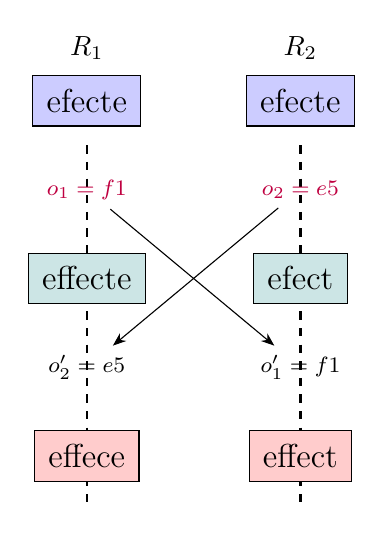
\begin{tikzpicture}[
	timeline/.style = {thick, dashed}, 
	>=Stealth, 
	send/.style = {>=Stealth, ->},
	list/.style = {rectangle, draw, inner sep = 5pt, outer sep = 2pt, fill = #1, font = \large},
	op/.style = {font = \footnotesize, #1}
  ]
  \uncover<2->{
    \node[list = blue!20, label = {above:{$R_1$}}] (r1) {efecte}; 
    \node[list = blue!20, right = 1.20cm of r1, label = {above:{$R_2$}}] (r2) {efecte};

    \foreach \r/\rbot in {r1/r1bot, r2/r2bot} {
      \node[below = 4.0cm of \r] (\rbot) {};
    }

    \draw[timeline] ($(r1.south)+(0,-5pt)$) -- ($(r1bot.south)+(0,-15pt)$);
    \draw[timeline] ($(r2.south)+(0,-5pt)$) -- ($(r2bot.south)+(0,-15pt)$);
  }

  \uncover<3->{
    \node (ins) [op = purple] at ($(r1)!0.25!(r1bot)$) {$o_1 = \ins{f}{1}$};
    \node (del) [op = purple] at ($(r2)!0.25!(r2bot)$) {$o_2 = \del{e}{5}$};

    \node (r11) [list = teal!20] at ($(r1)!0.50!(r1bot)$) {effecte};
    \node (r21) [list = teal!20] at ($(r2)!0.50!(r2bot)$) {efect};
  }

  \uncover<4->{
    \node (ins') [op] at ($(r2)!0.75!(r2bot)$) {$o_1' = \ins{f}{1}$};
    \node (del') [op] at ($(r1)!0.75!(r1bot)$) {$o_2' = \del{e}{5}$};

    \draw[send] (ins) -- (ins');
    \draw[send] (del) -- (del');

    \node (r12) [list = red!20] at ($(r1)!1.00!(r1bot)$) {effece};
    \node (r22) [list = red!20] at ($(r2)!1.00!(r2bot)$) {effect};
  }
\end{tikzpicture}
      \end{center}
    \column{0.40\textwidth}
      \begin{center}
	% file: tikz/ot-tcs06.tex

\newcommand{\ins}[2]{\textsc{Ins}(#1,#2)}
\newcommand{\del}[2]{\textsc{Del}(#2)}  % del(a, p): ignoring the deleted element ``a''

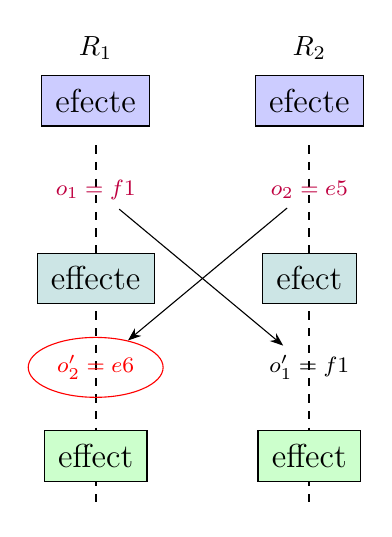
\begin{tikzpicture}[
	timeline/.style = {thick, dashed}, 
	>=Stealth, 
	send/.style = {>=Stealth, ->},
	list/.style = {rectangle, draw, inner sep = 5pt, outer sep = 2pt, fill = #1, font = \large},
	op/.style = {font = \footnotesize, #1}
  ]

  \uncover<5->{
    \node[list = blue!20, label = {above:{$R_1$}}] (r1) {efecte}; 
    \node[list = blue!20, right = 1.20cm of r1, label = {above:{$R_2$}}] (r2) {efecte};

    \foreach \r/\rbot in {r1/r1bot, r2/r2bot} {
      \node[below = 4.0cm of \r] (\rbot) {};
    }

    \draw[timeline] ($(r1.south)+(0,-5pt)$) -- ($(r1bot.south)+(0,-15pt)$);
    \draw[timeline] ($(r2.south)+(0,-5pt)$) -- ($(r2bot.south)+(0,-15pt)$);

    \node (ins) [op = purple] at ($(r1)!0.25!(r1bot)$) {$o_1 = \ins{f}{1}$};
    \node (del) [op = purple] at ($(r2)!0.25!(r2bot)$) {$o_2 = \del{e}{5}$};

    \node (r11) [list = teal!20] at ($(r1)!0.50!(r1bot)$) {effecte};
    \node (r21) [list = teal!20] at ($(r2)!0.50!(r2bot)$) {efect};
  }

  \uncover<6->{
    \node (ins') [op] at ($(r2)!0.75!(r2bot)$) {$o_1' = \ins{f}{1}$};
    \node (del') [op, red, ellipse, draw] at ($(r1)!0.75!(r1bot)$) {$o_2' = \del{e}{6}$};

    \draw[send] (ins) -- (ins');
    \draw[send] (del) -- (del');

    \node (r12) [list = green!20] at ($(r1)!1.00!(r1bot)$) {effect};
    \node (r22) [list = green!20] at ($(r2)!1.00!(r2bot)$) {effect};
  }
\end{tikzpicture}

      \end{center}
  \end{columns}
\end{frame}
%%%%%%%%%%%%%%%%%%%%

%%%%%%%%%%%%%%%%%%%%
\begin{frame}{}
  \begin{center}
    {\large Jupiter utilizes \red{OT}~\footnote{OT: Operational Transformation}~\ncite{Ellis:SIGMOD89} to achieve convergence.}
  \end{center}

  \begin{columns}[c]
    \column{0.50\textwidth}
      \fignocaption{width = 0.70\textwidth}{figs/ot-tcs06}
    \column{0.50\textwidth}
      \fignocaption{width = 0.65\textwidth}{figs/ot}
      \[
	\sigma; o_1; o_2' \equiv \sigma; o_2; o_1'
      \]
  \end{columns}
\end{frame}
%%%%%%%%%%%%%%%%%%%%

%%%%%%%%%%%%%%%%%%%%
\begin{frame}{}
  \centerline{\large OT functions for a replicated list object~\ncite{Ellis:SIGMOD89}}

  \resizebox{\textwidth}{!}{
    \begin{minipage}{\textwidth}
      % file: parts/list-ot.tex

\newcommand{\ldel}{\textsc{Del}}	% List DEL
\newcommand{\lins}{\textsc{Ins}}	% List INS
\newcommand{\ldelop}[2]{\ldel\left(#1, #2\right)}  % #1: index, #2: priority
\newcommand{\linsop}[3]{\lins\left(#1, #2, #3\right)}  % #1: index, #2: element, #3: priority

%%%%%%%%%% list-ot.tex %%%%%%%%%% 
\begin{align*}
  % ins vs. ins
  OT\Big(\lins(a_1, p_1, pr_1), \lins(a_2, p_2, pr_2)\Big) &= \begin{cases}
    \lins(a_1, p_1, pr_1) 		& p_1 < p_2 \\[3pt]
    \lins(a_1, p_1 + 1, pr_1) 		& p_1 > p_2 \\[3pt]
    \textsc{NOP} 			& p_1 = p_2 \land a_1 = a_2 \\[3pt]
    \lins(a_1, p_1 + 1, pr_1) 		& p_1 = p_2 \land a_1 \neq a_2 \land pr_1 > pr_2 \\[3pt]
    \lins(a_1, p_1, pr_1)		& p_1 = p_2 \land a_1 \neq a_2 \land pr_1 \le pr_2
  \end{cases} \\[10pt]
  % ins vs. del
  OT\Big(\lins(a_1, p_1, pr_1), \ldel(\_, p_2, pr_2)\Big) &= \begin{cases}
    \lins(a_1, p_1, pr_1) 		& p_1 \le p_2 \\[3pt]
    \lins(a_1, p_1 - 1, pr_1) 		& p_1 > p_2
  \end{cases} \\[10pt]
  % del vs. ins
  OT\Big(\ldel(\_, p_1, pr_1), \lins(a_2, p_2, pr_2)\Big) &= \begin{cases}
    \ldel(\_, p_1, pr_1) 		& p_1 < p_2 \\[3pt]
    \ldel(\_, p_1 + 1, pr_1) 		& p_1 \ge p_2
  \end{cases} \\[10pt]
  % del vs. del
  OT\Big(\ldel(\_, p_1, pr_1), \ldel(\_, p_2, pr_2)\Big) &= \begin{cases}
    \ldel(\_, p_1, pr_1) 		& p_1 < p_2 \\[3pt]
    \ldel(\_, p_1 - 1, pr_1) 		& p_1 > p_2 \\[3pt]
    \textsc{NOP}			& p_1 = p_2
  \end{cases} \\
\end{align*}
%%%%%%%%%% list-ot.tex %%%%%%%%%% 

    \end{minipage}
  }
\end{frame}
%%%%%%%%%%%%%%%%%%%%

%%%%%%%%%%%%%%%%%%%%
\begin{frame}{}
  \centerline{\large Consider a replicated system with $n \; (=3)$ clients.}

  \fignocaption{width = 0.50\textwidth}{figs/jupiter-schedule}
\end{frame}
%%%%%%%%%%%%%%%%%%%%

%%%%%%%%%%%%%%%%%%%%
\begin{frame}{}
  \begin{Theorem}[Equivalence of CJupiter and Jupiter]
    Under the same schedule, the behaviors of corresponding replicas in CJupiter and Jupiter are the same.
  \end{Theorem}

  \vspace{0.30cm}
  \centerline{\large At the server side:}
  \begin{prop}[$n \leftrightarrow 1$ (Informal)]
    The single $n$-ary ordered state space at the server side in CJupiter 
    is a \red{compact representation} of $n$ $2D$ state spaces at the server side in Jupiter.
  \end{prop}

  \vspace{0.30cm}
  \centerline{\large At the client side:}
  \begin{prop}[$1 \leftrightarrow 1$ (Informal)]
    Jupiter is \red{slightly optimized in implementation} at clients by eliminating redundant OTs than CJupiter.
  \end{prop}
\end{frame}
%%%%%%%%%%%%%%%%%%%%


\end{document}
%%%%%%%%%%